\begin{enumerate}
\item See the attached R code for the data normalization and splits.
\item We applied the best subset selection on the training set. Figure 1 shows the curves for $R^2$, adjusted $R^2$, $C_p$ and BIC as a function of the number of predictors. As expected $R^2$ increases as the number of predictors increases. Adjusted $R^2$ and $C_p$ both suggest that models with 7 predictors would be the best model, since these models have the highest adjusted $R^2$ and lowest $C_p$. These two also show that a model with 6 predictors will achieve about the same performance. BIC replaces the penalty term used by $C_P$ ,$2d\hat{\sigma}^2$, with $log(n)d\hat{\sigma}^2$, where $n$ is the number of observations. Since $log(n) > 2$ for any $n >7$, BIC places a heavier penalty of models with more predictors. This can be observed in Figure 1, where the BIC statistic suggests a model with 2-4 predictors is best.  We'll choose 7 feature model. Figure 2 shows the the selected features used for the best model for the range of predictors. In our selected model the features used are all the features except \textit{gleason} .  The \textbf{training error} for this model is 0.439. The \textbf{test error} is 0.516. 
\newline
\begin{figure}[htbp]
\centering
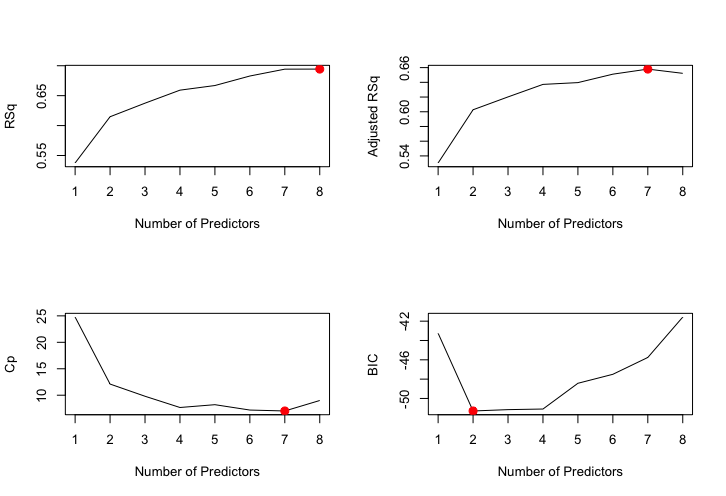
\includegraphics[scale=0.7]{Best_subset.png}
\caption{RSq, adjusted RSq, Cp and BIC values versus the number of predictors in best subset selection.}
\end{figure}
\newline
\begin{figure}[htbp]
\centering
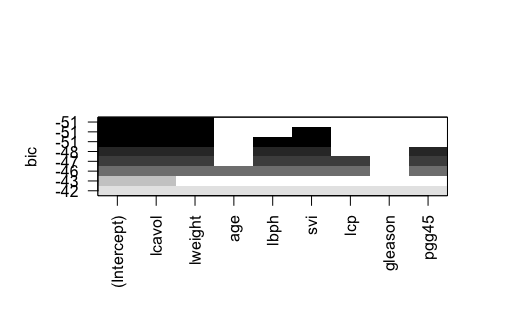
\includegraphics[scale=0.7]{Features.png}
\caption{Selected features for best model with predictors from BIC statistic.}
\end{figure}
\item Figure 3 shows the values of the coefficients in relation to $\lambda$ for the ridge regression fit on the training data. The results are as expected. On the left hand side $\lambda$ is almost zero, therefore the ridge coefficient estimates are essentially the same as the least squares estimates. As $lambda$ increases the coefficient estimates shrink to zero. On the right hand side of the plot, when $lambda$ is large, all of the estimates are zero.
\newline
\begin{figure}[htbp]
\centering
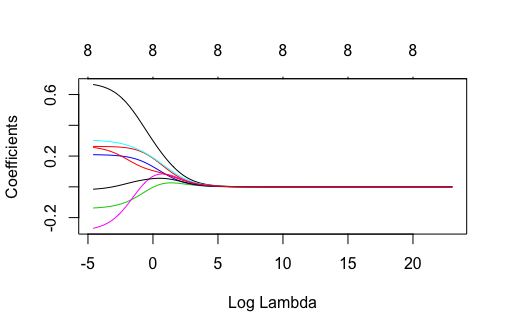
\includegraphics[scale=0.7]{Ridge.png}
\caption{Ridge regression coefficients in relation to $lambda$.}
\end{figure}
\item See code for 5-fold cross-validation for the ridge regression model. For this model the \textbf{training error} in MSE is 0.10586, and the \textbf{test error} is 0.44623. 
\item Figure 4 shows the plot of the lasso coefficient estimates plotted against $\lambda$. In lasso the coefficients shrink to zero as $\lambda$ gets sufficiently large, which can be seen in Figure 4. This is in contrast to ridge regression, where the coefficients approach but never shrink to zero.
\newline 
\begin{figure}[htbp]
\centering
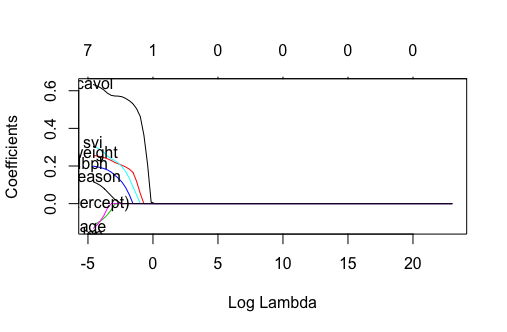
\includegraphics[scale=0.7]{Lasso.png}
\caption{Lasso coefficients in relation to $lambda$.}
\end{figure}
\item See the code for 5-fold cross-validation for the lasso model. For this model the \textbf{training error} is 0.10342, and the \textbf{test error} is 0.4426. In ridge regression all off the coefficients are used, but the lasso coefficients are significantly smaller. In fact, many of the lasso coefficients, such as svi and lcp, are, for practical purposes, zero. Since lasso coefficients are generally a more sparse representation, since they go to zero, this is expected. The ridge regression coefficients and the lasso coefficients are:
\newline
\begin{tabular}{{c|c|c}}
 & ridge & lasso \\
 \hline
 lcavol & -0.6361918 & -1.157344e-04 \\
 lweight & -0.2638188 & -7.258686e-05 \\
 age & 0.1315373 & -3.758792e-05 \\
 blph & -0.2072106 & -4.337587e-05 \\
 svi & -0.3251784 & -9.135083e-05 \\
 lcp & 0.1615693 & -8.125745e-05 \\
 gleason & -0.1387185 & -5.804440e-05
\end{tabular}
\item The linear regression model trained on all the features has a higher MSE than the ridge regression and lasso models trained with cross-fold validation. The training error and test error is shown below, along with the error from the ridge regression and lasso cross-validation errors:
\newline
\begin{tabular}{{c|c|c|}}
 & train error & test error \\
 \hline
 ridge CV & 0.10586 & 0.44623 \\
 lasso CV & 0.10342 & 0.4436 \\
 linear & 0.43919 & 0.5212 \\

\end{tabular}
\end{enumerate}